\section{Experiment Setup and Evaluation}
In this section, we will present our experiment setup, the evaluation metrics, analyze the results, and do error analysis.

\subsection{Experiment Setup}
The model is divided into two parts. We have implemented our model on PyTorch.

\subsubsection{Tweet Classifier}
We have used a Long short-term memory (LSTM) model. LSTM is a variant of Recurrent neural network (RNN). This classifier predicts whether the tweet may contain medication name or not. The model transforms the tweet text into it's vector representation using Glove Twitter word embeddings~\footnote{glove.twitter.27B.100d: ~\url{https://pytorch.org/text/_modules/torchtext/vocab.html}}. We generate vocab of training dataset with minimum frequency three. This model uses two Rectified Linear Unit (ReLU) and one linear-classification for prediction. The model design is shown in figure~\ref{fig:model-imran}. We have used Adam optimizer and Sigmoid loss function.

\begin{figure}[h]
	\centering
	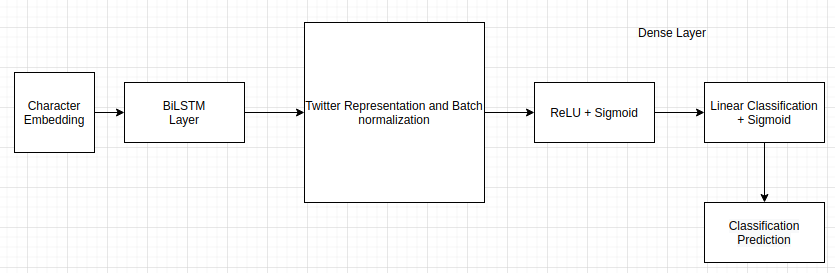
\includegraphics[width=0.99\linewidth]{Figures/model.png}
	\caption{Architecture of the model}
	\label{fig:model-imran}
\end{figure}

\subsubsection{Span Detection}
For a positive class tweet, we searched a medication name with our pre-compiled medication and dietary list. 

\subsection{Evaluation Metrics}
BioCreative mentioned f1-score for positive class as a evaluation metric. However, we have added precision, and recall as well for comparison.

\subsection{Results and Discussion}
For our dataset 1 which is most extremely imbalanced with only 0.38\% positive class, The f1-score of positive class is 0.60. As we increased the size of positive classes, the f1-score of positive class also improved. The f1-score is 0.90 and 0.94 respectively for dataset 2 and dataset 3. From the table~\ref{table:3}, we can find that precision and recall improve as well. A model developed for highly imbalanced dataset performs better for more balanced dataset for a similar task of detecting tweets in medication names is also supported by Weissenbacher et al.~\cite{weissenbacher2019deep}.

\begin{table}[h!]
	\centering
	\begin{tabular}{||c c c c c c||} 
		\hline
		Dataset & Positive-class & F1-score & Precision & Recall & TP/FP/FN \\ [0.5ex] 
		\hline\hline
		Dataset 1 & 200 & 0.60 & 0.70 & 0.53 & 26/11/23 \\ 
		Dataset 2 & 500 & 0.90 & 0.95 & 0.85 & 105/5/19 \\
		Dataset 3 & 1000 & 0.94 & 0.97 & 0.91 & 229/8/23 \\
		\hline
	\end{tabular}
	\caption{Evaluation of the model on test data}
	\label{table:3}
\end{table}

We have performed a competitive analysis on dataset 2 about parameter tuning (see table~\ref{table:4}). The three key area of parameter tuning are: batch size, embedding, and batch normalization. With dataset being extremely imbalanced, setting up the right batch size is important. From the table~\ref{table:4}, we can see that f1-score decreases when batch size is too low or too high. Secondly, embedding tuning improved the performance. When embedding dimension is too high or too low, f1-score decreases as well. The other technique which helped to improve performance, is batch normalization. This is possibly because our dataset is highly imbalanced and batch normalization improves the performance of imbalanced dataset. A recent study~\cite{kocaman2020improving} also shows this.

\begin{table}[h!]
	\centering
	\begin{tabular}{||c c c c c||} 
		\hline
		Dataset & Batch Size & Embedding & Batch Normalization & F1-score\\ [0.5ex] 
		\hline\hline
		Dataset 2 (default) & 128 & glove (100d) & yes & 0.90 \\
		\hline
		Dataset 2 & 128 & glove (100d) & no & 0.89 \\
		\hline
		Dataset 2 & 32 & glove (100d) & yes & 0.86 \\
		\hline
		Dataset 2 & 64 & glove (100d) & yes & 0.87 \\
		\hline
		Dataset 2 & 256 & glove (100d) & yes & 0.82 \\
		\hline
		Dataset 2 & 128 & glove (200d) & yes & 0.82 \\
		\hline
		Dataset 2 & 128 & glove (200d) & no & 0.86 \\
		\hline
		Dataset 2 & 128 & glove (50d) & yes & 0.84 \\
		\hline
		Dataset 2 & 128 & glove (50d) & no & 0.85 \\
		\hline
	\end{tabular}
	\caption{Evaluation of the model on various parameters tuning over dataset 2}
	\label{table:4}
\end{table}


\subsection{Error Analysis}

From the table~\ref{table:3}, for dataset 2, there are five false positive cases. we will compare our model with Weissenbacher et al.~\cite{weissenbacher2019deep}'s eight error category for false positive case for their Kusuri model of similar task: Medical topic, Weighted words/patterns, Ambiguous name, Food topic, Insufficient context, Cosmetic topic, Unknown, Error annotation.

These five cases are listed on table~\ref{table:5}. If we look through the cases, the number five contains medication name such as `Codeine'. This was marked as negative class by the annotators. Possibly this is an annotation error. In the other cases, tweets contain words such as food terms (crips, carbs), words often associated with medical topics (meds, cuts, relaxer), ambiguous terms (Prenatal). As medical tweets often describe symptoms and associated with generic medical terms (such as cough, flu, doctor, vitamin, meds, etc), it often confuses the classifier.

\begin{table}[h!]
	\centering
	\begin{tabular}{||c c||} 
		\hline
		Number & Tweet \\ [0.5ex] 
		\hline\hline
		1 & The after fact of having a C section Lawd when the meds ware off I actually feel cut open \\ \hline
		2 & I need crisps and carbs \\ \hline
		3 & I want a relaxer... and a blunt cut... \\ \hline
		4 & My child is apparently auditioning for So You Think You Can Dance: Prenatal Edition. I think he's got a real shot at the title. \\ \hline
		5 & I'm a suckah For Codeine \\ \hline
	\end{tabular}
	\caption{False positive cases of dataset 2}
	\label{table:5}
\end{table}

From the table~\ref{table:3}, for dataset 2, there are nineteen false negative cases. we will compare our model with Weissenbacher et al.~\cite{weissenbacher2019deep}'s six error category for false negative case: Ambiguous name, Drug not/rarely seen, Generic terms, Nonmedical topic, Short tweets, Error annotation.

These nineteen cases are listed on table~\ref{table:6}. If we look through the cases, there are ambiguous name in six (12, 13, 14, 15, 17, 19) cases, Drug not/rarely seen in six (1, 2, 3, 5, 9, 10) cases, Generic terms in three (4, 6, 18) cases, Nonmedical topic in one (16) case, and Error annotation in three (7, 8, 11) cases. The cause of false negative mostly mirrors to false positives.
 
\begin{table}[h!]
	\centering
	\begin{tabular}{||c m{50em}||} 
		\hline
		Number & Tweet \\ [0.5ex] 
		\hline\hline
		1 & @user thanks, I'm 16wks \& still taking diclectin... so eventually I'll feel wonderful :) \\ \hline
		2 & Gaviscon is my new best friend \\ \hline
		3 & But I do carry a Flonase spray in my purse faithfully bc I have	the worst 
		sinus/respiratory infections which cause me to be dizzy \\ \hline
		4 & @user Try generic (Wal-Mart brand) Prilosec OTC gel capsules. It's the ONLY thing that has helped with my pregnancy \\ \hline
		5 & @user Hey! He is sleep... still has a Lil anesthesia... but had 2 bottles of Pedialyte and hasn't thrown up... might be home today \\ \hline
		6 & So I'm watching this commercial about Symbicort inhaler, which I use because I have asthma, and let me tell yall \\ \hline
		7 & @user @user Got my Tdap at 37 weeks... Hope it wasn't too late. Article states 27-36 weeks. \\ \hline
		8 & Last time I had a sore arm from a vaccine was when I got my meningitis vaccine \\ \hline
		9 & A whole 24hrs of me just being itchy af and its nothing I can do about it. Benadryl don't fuckin work g \\ \hline
		10 & I'm so uncomfortable.. Tylenol3 is my best friend tonight. Gonna snuggle my hubby \& crash. \\ \hline
		11 & Staying in the hospital tonight.Diagnosed with preeclampsia.Was given shotsto make her lungs grow faster, and hoping she stays baking longer \\ \hline
		12 & My 4th Rhogam shot hurt just as bad as my 1st one. O negative blood is a blessing \& a curse. [...] \\ \hline
		13 & @user how was I supposed to know? It's one full bottle and a few pills in the other. Gotta find them. You can have them. \\ \hline
		14 & I hate the sleepy side effect when your eggo is preggo or maybe it these vitamins.never wear panties ever but I... http://t.co/vQnof2HBx3 \\ \hline
		15 & Last min oxys so i can sleep... juju knocked... and rell at home cleaning lol \\ \hline
		16 & Stephanie sounds like she needs some decongestant! [...] \\ \hline
		17 & @user I am. We are going through 14pts a week \& I'm pretty much the only person who has any. And orange Rennies. It's just blurgh. \\ \hline
		18 & My diet consists of adderall for breakfast, beer for dinner, \& cake pops for bed time snack. So I should be skinny again soon. \\ \hline
		19 & prenatals have done wonders to my hair \\ \hline
	\end{tabular}
	\caption{False negative cases of dataset 2}
	\label{table:6}
\end{table}